\section{Introduction}

\subsection*{Context}

This project starts an extension of work done in a previous project by Sewen Thy and
Ilya Sergey, in which they theorised and then implemented the beginnings of an
automated ``Extract Method'' refactoring tool for the Rust programming language.
Extract Method refactorings are a well known and widely used refactoring
approach, however, due to Rust's unique approach to memory safety of of
ownership and borrowing, and the lifetime system that enforces these rules, it
is far more difficult to implement than in other languages. Ilya Sergey et al's
contribution focused on the theoretical apects of the problem
\cite{AdventureOfALifetime}, whilst Sewen Thy's contribution focused on the
implementation, \cite{BorrowingWithoutSorrowing}, with a pure Rust algorithm and
a heavy reliance on Intellij IDEA's type inference and static code analysis
tools. Their approach was dubbed ``Rusty Extraction Maestro'' (REM). Figure
\ref{fig:rem-overview} gives a high-level overview
of the REM algorithm.

\begin{figure}[h]
    \centering
    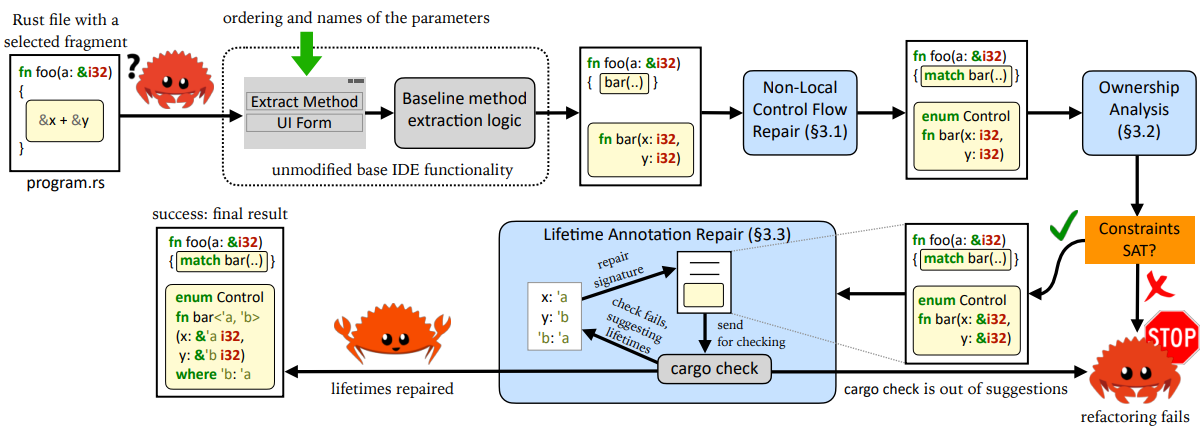
\includegraphics[width=\columnwidth]{Figures/rem-overview.png}
    \caption{An overview of the REM Algorithm, from \cite{AdventureOfALifetime}}
    \label{fig:rem-overview}
\end{figure}

The REM algorithm is a three stage process, beginning after Intellij IDEA has
performed an initial code extraction and type inference. If REM fails (i.e. an
extraction isn't possible), then the code is returned to its original condition.
The stages are:

\begin{enumerate}
    \item \textbf{Controller:} handles any non local control flow. This includes
    \textcolor{blue}{return}, \textcolor{blue}{break} and
    \textcolor{blue}{continue}. As rust is an expressions based language
    \cite{rbooka} these statements can be used in arbitrary
    combinations, adding substantial complexity. The algorithm is included appendix
    \ref{app:non_local_control_flow_repair}.
    \item \textbf{Borrower:} infers any ownership annotations. In Rust,
    variables can be either immutable (imm) or mutable (mut). Additionally, they
    are either owned by the current scope, or borrowed from another scope.
    \inputminted[linenos, tabsize=2]{rust}{snippets/borrow.rs}
    The borrower is at its core, a dataflow analysis algorithm that infers the ownership of each
    variable, and adds the correct information to the function body and scope.
    The algorithms are included in appendix \ref{app:ownership_and_borrowing_repair}.
    \item \textbf{Repairer:} focuses on correcting lifetime annotations in Rust
    functions, particularly those involving references. When a function has
    borrowed values, lifetimes need to be explicitly managed to ensure that the
    references remain valid. The repairer first explicitly annotates all
    lifetimes, using the rust compiler (rustc) to check for errors: \verb|'a|
    represents the lifetime of \verb|x| \footnote{See
    \href{https://doc.rust-lang.org/nomicon/lifetimes.html}{Rust Book - Lifetimes} for more information}.
    \inputminted[]{rust}{snippets/lifetime.rs}
    It then applies the lifetime elision rules \cite{rbookb} to remove any
    lifetimes the compiler can infer to bring the code back to a human readable
    state.
    The algorithm is included in appendix \ref{app:lifetime_repair}
\end{enumerate}

One of the most difficult aspects of any refactoring / optimisation tool is
ensuring the correctness of the output. A refactor is ``correct'' if the orginal
behaviour of the program is preserved \cite{ProvingCompilerOptimisations}.
Unfortunately, for the REM algorithm, formal verification of the correctness is
impossible as it would a model of the formal semantics of (safe) Rust, which
doesn't exist \footnote{Formal correctness proofs for refactorings are very
rare, even for languages with fully formalised semantics
\cite{AdventureOfALifetime}}. Instead, the toolchain relies on a combination of
extensive testing, the rust compiler, and a fail-early approach to ensure that
the user is never presented with ``incorrect'' code.

\subsection*{Aims}

This project aims to improve and extend on the REM tool by addressing key
limitations and researching (and subsequently implementing) new approaches to
refactoring.
\begin{enumerate}
    \item \textbf{Fixing REM's Issues:} Remove the dependency on (\textit{i})
    \verb|rustc| and (\textit{ii}) Intellij IDEA to make REM a standalone tool.
    Additionally, reduce file I/O overhead by optimising the tools internal data
    handling
    \item \textbf{Platform-Agnostic Code Extraction:} Build a complete,
    end-to-endsolution for method extraction using \textit{Rust Analyzer} (RA)
    for the code extraction, wrapped in a single, user-friendly CLI tool written
    entirely in Rust.
    \item \textbf{VSCode Extension Proof of Concept:} Develop a VSCode extension
    to showcase how REM can be easily integrated into editors, with potential
    for extending to other environments.
    \item \textbf{Exploring New Refactorings:} The big ticket item for this
    research project where the bulk of my time will be spent, investigating
    extract method refactoring for the far more advanced areas of
    \textit{Generics, Ansynchronous Code, Macros, Closures, and Const
    Functions}. \textit{Generics} and \textit{Asynchronous Code} present special
    challenges due to (a) the complex lifetimes and (b) the uncertainty of the
    code at compile time, and are what the majority of the research will focus
    on.
    \item \textbf{Final Aim: Merging REM with RA:} An ultimate, ambitious goal
    for this project is to merge the REM toolchain with RA, Rust's official
    language server protocol (LSP) implementation
    \footnote{https://rust-analyzer.github.io/}. This would require proving
    substantially more of the correctness of REM (although as previously noted,
    a full correctness proof is impossible), allowing its functionality to be
    available across any Rust-supported editor. If that is not feasible, then a
    well featured VSCode extension is a suitable alternative.
\end{enumerate}